%%
%%  Department of Electrical, Electronic and Computer Engineering.
%%  EPR400/2 Final Report - Main File.
%%  Copyright (C) 2011-2021 University of Pretoria.
%%

\documentclass{epr400}

%% EDIT: Replace the following with your information.
\eprtitle{A Smart Green EPR400 Final Report LaTeX digital twin}
\eprcode{EPR402}
\eprcandidatename{P. Pompies}
\eprstudentnumber{12345678}
\eprdate{November 2023}
\eprsupervisor{Mr. X. Why}
\eprcopynum{Electronic copy}

\begin{document}

%% Generate the required title page.
\maketitlepage

%% --- PART 1 ------------------------------------------------------------

\pagestyle{plain}
\pagenumbering{roman}

\eprsec{Part 1. Preamble}

\vspace*{0.5cm}

%% Import the required preamble pages.
%%
%%  Department of Electrical, Electronic and Computer Engineering.
%%  EPR400/2 Final Report - Preamble.
%%  Copyright (C) 2011-2021 University of Pretoria.
%%

This report describes work that I have completed in my final year project, developing a laser pointer turret based mosquito air defence system.
\\[2ex]
\textit{Project proposal and technical documentation} \newline
This main report contains an unaltered copy of the approved Project Proposal (as Part 2 of the report).

Technical documentation appears in Part 4 (Appendix).

All the code that I developed appears as a separate submission on the AMS.
\\[2ex]
\textit{Project history} \newline
This project does not extend on a previous project. The design and implementation is completely new.

I used library code for low level hardware interfacing with camera and motors. The implementation of the Hungarian algorithm was taken from an existing software module. The rest of the work reported on here, is entirely my own.
\\[2ex]
\textit{Language editing} \newline
This document has been language edited by a knowledgeable person. By submitting this document in its present form, I declare that this is the written material that I wish to be examined on.

My language editor was Ms. Michelle Hartman.

\vspace*{0.5cm}

\begin{tabular}{cp{4cm}ll}
  
\includegraphics[width=3.5cm]{figures/mich_handtekening.png} &  & \underline{\today} \\
  \textit{Language editor signature}                           &  & \textit{Date}
\end{tabular}

\vspace*{0.5cm}

\textit{Declaration}
\\[2ex]
I, \underline{\eprthecandidatename} understand what plagiarism is and have carefully studied the plagiarism policy of the University. I hereby declare that all the work described in this report is my own, except where explicitly indicated otherwise. Although I may have discussed the design and investigation with my study leader, fellow students or consulted various books, articles or the internet, the design/investigative work is my own. I have mastered the design and I have made all the required calculations in my lab book (and/or they are reflected in this report) to authenticate this. I am not presenting a complete solution of someone else.

Wherever I have used information from other sources, I have given credit by proper and complete referencing of the source material so that it can be clearly discerned what is my own work and what was quoted from other sources. I acknowledge that failure to comply with the instructions regarding referencing will be regarded as plagiarism.  If there is any doubt about the authenticity of my work, I am willing to attend an oral ancillary examination/evaluation about the work.

I certify that the Project Proposal appearing as the Introduction section of the report is a verbatim copy of the approved Project Proposal.

\begin{tabular}{cp{5cm}ll}
  
\includegraphics[width=3.5cm]{figures/anton_handtekening.png} &  & \underline{\today} \\
  \eprthecandidatename                                          &  & Date
\end{tabular}

%% End of File.


\newpage

%% Add the Table of Contents.
\makeatletter
\renewcommand\@dotsep{200}
\makeatother
\tableofcontents
\thispagestyle{empty}
\newpage

%% Import the required abbreviation pages.
%%
%%  Department of Electrical, Electronic and Computer Engineering.
%%  EPR400/2 Final Report - Abbreviations.
%%  Copyright (C) 2011-2021 University of Pretoria.
%%

% \section*{LIST OF ABBREVIATIONS}

% \begin{tabular}{p{3cm}l}
%     \textbf{AWGN} & Additive white Gaussian noise           \\
%     \textbf{BER}  & Bit error rate                          \\
%     \textbf{BPSK} & Bipolar phase shift keying              \\
%     \textbf{DSP}  & Digital signal processor                \\
%     \textbf{GSM}  & Global System for Mobile communications \\
%     \textbf{SNR}  & Signal-to-noise-ratio                   \\
% \end{tabular}


%% End of File.

\newacronym{mads}{MADS}{mosquito air defence system}
\newacronym{pid}{PID}{proportional-integral-derivative}
\newacronym{gpio}{GPIO}{general purpose input/output}
\newacronym{rpm}{RPM}{revolutions per minute}
\newacronym{gpu}{GPU}{graphics processing unit}
\newacronym{cpu}{CPU}{central processing unit}
\newacronym{led}{LED}{light emitting diode}
\newacronym{rgb}{RGB}{red, green, blue}
\newacronym{ccl}{CCL}{connected components labelling}
\newacronym{sort}{SORT}{simple online and real-time tracking}
\newacronym{cuda}{CUDA}{compute unified device architecture}
\newacronym{mipi}{MIPI}{mobile industry processor interface}
\newacronym{csi}{CSI}{camera serial interface}
\newacronym{usb}{USB}{universal serial bus}
\newacronym{pwm}{PWM}{pulse width modulation}
\newacronym{cad}{CAD}{computer aided design}

\newpage

%% --- PART 2 ------------------------------------------------------------

\eprsec{Part 2. Project definition: approved Project Proposal}

This section contains the problem identification in the form of the complete approved Project Proposal, unaltered from the final approved version that appears on the AMS.

\newpage

%% Import the approved project proposal
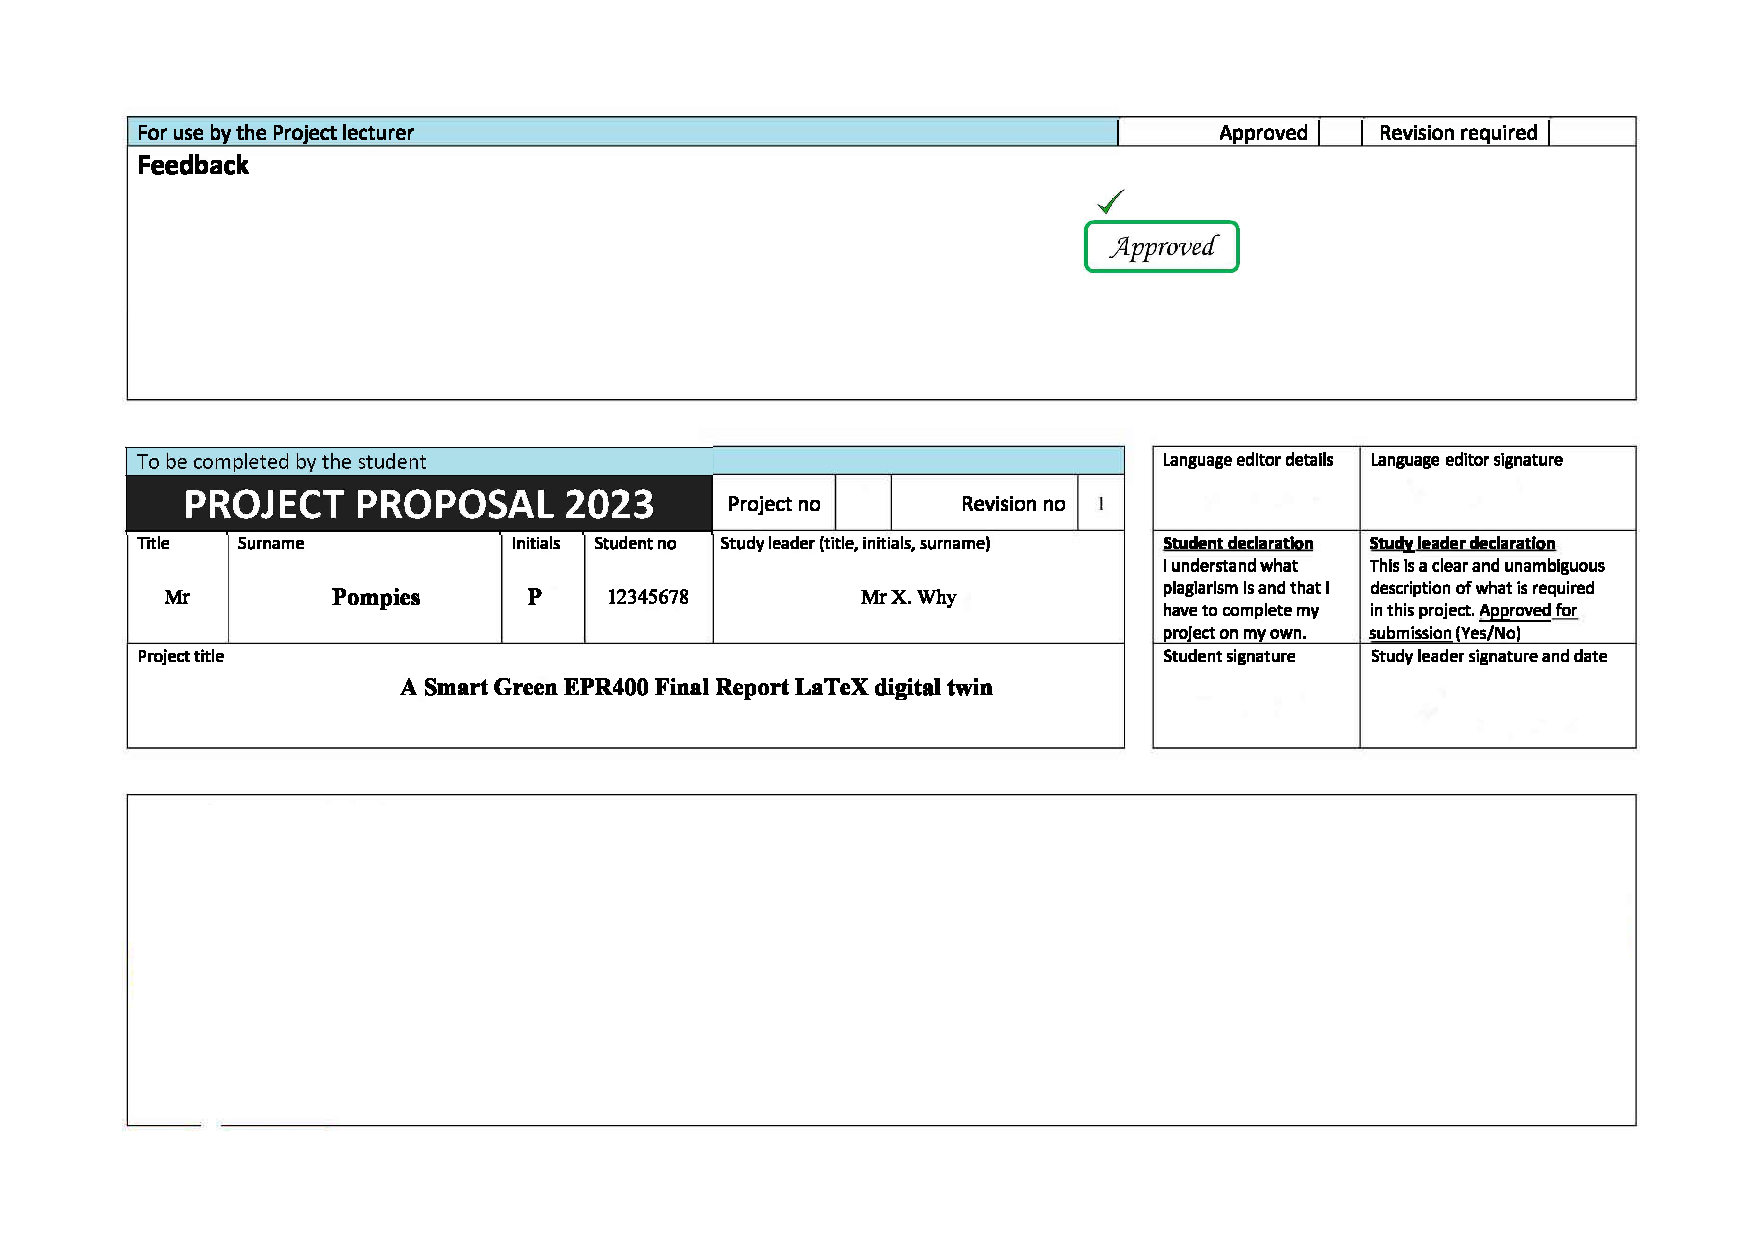
\includepdf[pages=-, angle=90]{ApprovedProposal.pdf}

\addtocontents{toc}{\protect\contentsline{subsection}{1. Project description}{}\%}
\addtocontents{toc}{\protect\contentsline{subsection}{2. Technical challenges in this project}{}\%}
\addtocontents{toc}{\protect\contentsline{subsection}{3. Functional analysis}{}\%}
\addtocontents{toc}{\protect\contentsline{subsection}{4. System requirements and specifications}{}\%}
\addtocontents{toc}{\protect\contentsline{subsection}{5. Field conditions}{}\%}
\addtocontents{toc}{\protect\contentsline{subsection}{6. Student tasks}{}\%}

%% --- PART 3 ------------------------------------------------------------

\eprsec{Part 3. Main Report}
\newpage

%% Reset the page number style and count.
\pagenumbering{arabic}
\setcounter{page}{1}

%% Import the main report content
%%
%%  Department of Electrical, Electronic and Computer Engineering.
%%  EPR400/2 Final Report - Section 1.
%%  Copyright (C) 2011-2021 University of Pretoria.
%%

\section{Literature study}

Shannon {\it et al.}\cite{Shannon:A_Mathematical_Theory_of_Communications}


\newpage

%% End of File.



%%
%%  Department of Electrical, Electronic and Computer Engineering.
%%  EPR400/2 Final Report - Section 2.
%%  Copyright (C) 2011-2021 University of Pretoria.
%%

\section{Approach}


\newpage

%% End of File.


%%
%%  Department of Electrical, Electronic and Computer Engineering.
%%  EPR400/2 Final Report - Section 3.
%%  Copyright (C) 2011-2021 University of Pretoria.
%%

\section{Design and implementation}

\subsection{Design summary}

\subsection{Theoretical analysis and modelling}

\subsection{Simulation study and optimisation}

\subsection{Hardware design}

\subsection{Hardware implementation}

\subsection{Software design}

\subsection{Software implementation}

\subsection{Final system integration and testing}

\newpage

%% End of File.


%%
%%  Department of Electrical, Electronic and Computer Engineering.
%%  EPR400/2 Final Report - Section 4.
%%  Copyright (C) 2011-2021 University of Pretoria.
%%

\section{Results}

\subsection{Summary of results achieved}

\subsection{Qualification tests}

\newpage

%% End of File.



%%
%%  Department of Electrical, Electronic and Computer Engineering.
%%  EPR400/2 Final Report - Section 5.
%%  Copyright (C) 2011-2021 University of Pretoria.
%%

\section{Discussion}

\subsection{Critical evaluation of the design}

\subsubsection{Interpretation of results}

\subsubsection{Critical evaluation}

\subsubsection{Unsolved problems}

\subsubsection{Strong points of the design}

\subsubsection{Expected failure conditions}

\subsection{Considerations in the design}

\subsubsection{Ergonomics}

\subsubsection{Health and safety}

\subsubsection{Environmental impact}

\subsubsection{Social and legal impact}

\subsubsection{Ethics clearance}

\newpage

%% End of File.



%%
%%  Department of Electrical, Electronic and Computer Engineering.
%%  EPR400/2 Final Report - Section 6.
%%  Copyright (C) 2011-2021 University of Pretoria.
%%

\section{Conclusion}

\subsection{Summary of the work completed}

\subsection{Summary of the observations and findings}

\subsection{Contribution}

\subsection{Future work}

\newpage

%% End of File.




%% Use the IEEE Transactions style for the references.
\bibliographystyle{IEEEtran}
\bibliography{finalreport}
\newpage

%% --- PART 4 ------------------------------------------------------------

\eprsec{Part 4. Appendix: technical documentation}
\newpage

\setcounter{secnumdepth}{0}

\titleformat{\subsection}[display]
{\fontsize{14pt}{16.8pt}\selectfont\bfseries} {} {5pt} {\formatsubsectiontitle}
\titleformat{\subsection}[display]
{\fontsize{14pt}{16.8pt}\selectfont\bfseries} {} {5pt} {\formatsubsectiontitle}

%%
%%  Department of Electrical, Electronic and Computer Engineering.
%%  EPR400/2 Final Report - Technical Documentation.
%%  Copyright (C) 2011-2021 University of Pretoria.
%%

\section{HARDWARE part of the project}

\subsection{Record 1. System block diagram}
\begin{figure}[H]
  \centering
  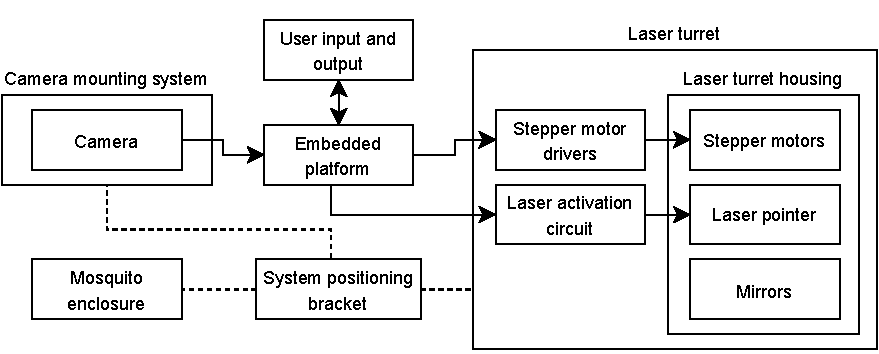
\includegraphics[width=\textwidth]{figures/hardware_block_diagram.pdf}
  \caption{System block diagram.}
\end{figure}


\subsection{Record 2.  Systems level description of the design}


\subsection{Record 3. Complete circuit diagrams and description}


\subsection{Record 4. Hardware acceptance test procedure}


\subsection{Record 5. User guide}


%% --------------------------------------------------------------------

\section{SOFTWARE part of the project}

\subsection{Record 6. Software process flow diagrams}
\begin{figure}[h]
  \centering
  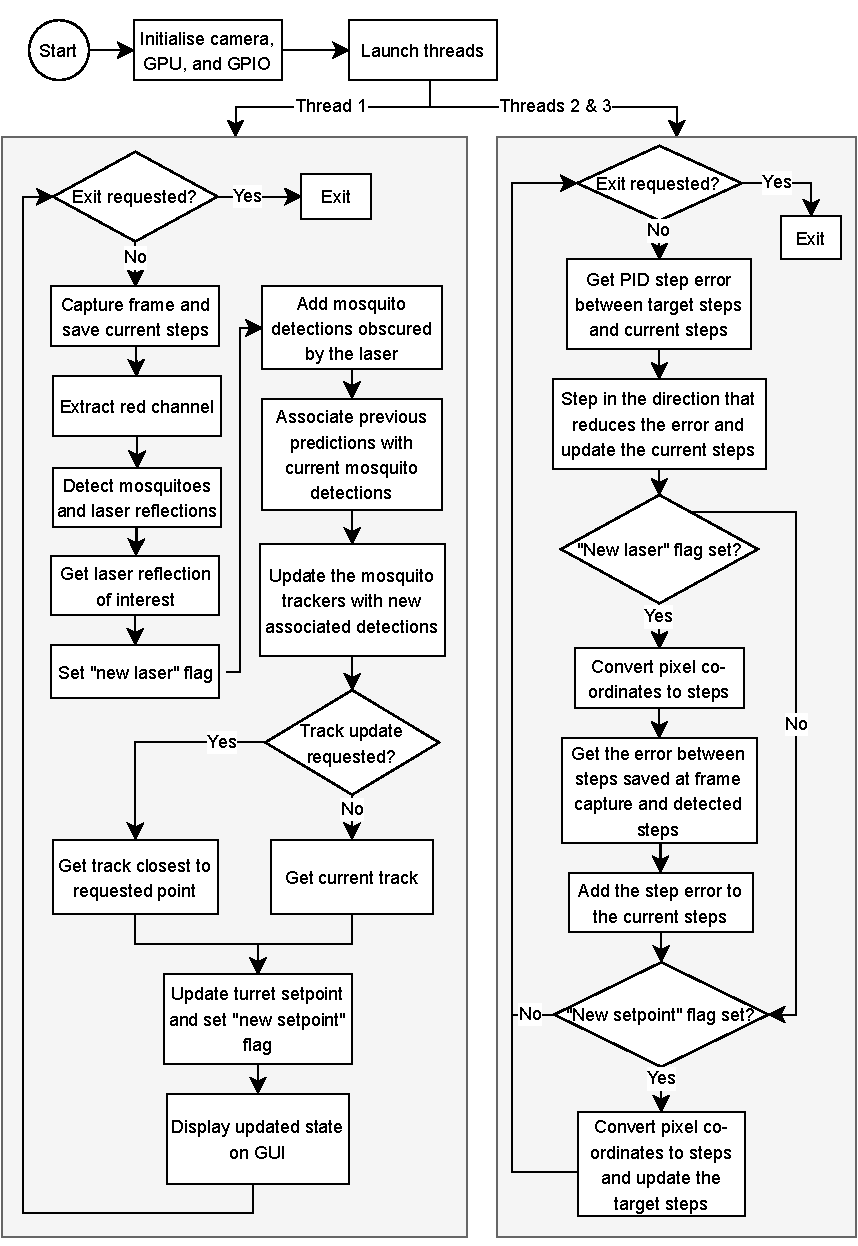
\includegraphics[width=0.95\textwidth]{figures/software_flow_diagram.pdf}
  \caption{Software flow diagram.}
\end{figure}


\subsection{Record 7. Explanation of software modules}


\subsection{Record 8. Complete source code}
Complete code has been submitted separately on the AMS.


\subsection{Record 9. Software acceptance test procedure}


\subsection{Record 10. Software user guide}


%% --------------------------------------------------------------------

\section{EXPERIMENTAL DATA}

\subsection{Record 11. Experimental data}


%% End of File.




\end{document}

%% End of File.
